\documentclass[a4paper,landscape,8pt]{article}
\usepackage[utf8]{inputenc}
\usepackage{fullpage}
\usepackage{listings}
\usepackage{pdflscape}
\usepackage[left=0.5cm,top=1cm,right=0.5cm,bottom=2cm,bindingoffset=0.5cm,a4paper,landscape]{geometry}
\usepackage{tocloft}
\usepackage{titlesec}
\usepackage{mdwlist}
\usepackage{amsmath}
\usepackage{color}
\usepackage{multicol}
\usepackage{fancyhdr}
\usepackage{graphicx}
\newcommand{\BigO}[1]{\ensuremath{\operatorname{O}\bigl(#1\bigr)}}
\setlength{\tabcolsep}{0mm}

\definecolor{dkgreen}{rgb}{0,0.6,0}
\definecolor{gray}{rgb}{0.5,0.5,0.5}
\definecolor{mauve}{rgb}{0.58,0,0.82}
\lstset{
         basicstyle=\footnotesize\ttfamily,
         keywordstyle=\color{blue},          % keyword style
         commentstyle=\color{dkgreen},       % comment style
         stringstyle=\color{mauve},         % string literal style
         %numbers=left,
         %numberstyle=\tiny,
         numbersep=5pt,
         tabsize=2,
         extendedchars=true,
         breaklines=true,
         showspaces=false,
         showtabs=false,
         showstringspaces=false
         xleftmargin=10pt,
         framexleftmargin=10pt,
         framexrightmargin=5pt,
         framexbottommargin=6pt,
}

\setcounter{secnumdepth}{-2} % Ignore numbering on sections
\renewcommand{\cftsecleader}{\cftdotfill{\cftdotsep}} % Dots on sections

% {cmd}{left spacing}{before spacing}{after spacing}
\titlespacing\section{0pt}{4pt plus 2pt minus 2pt}{2pt plus 2pt minus 2pt}
\titlespacing\subsection{0pt}{0pt plus 2pt minus 2pt}{0pt plus 2pt minus 2pt}

\titleformat{\section}{\large\bfseries}{\thesection}{10pt}{}
\titleformat{\subsection}{\bfseries}{\thesection}{8pt}{}

\setlength{\tabcolsep}{5pt}
\setlength{\headheight}{9pt}
\setlength{\headsep}{9pt}

\fancypagestyle{tcr}{%
  \fancyhf{} %clear all headers and footers fields
  \fancyhead[R]{\thepage}
  \fancyhead[L]{\textbf{Linköping University}}
  \renewcommand{\headrulewidth}{0.4pt}
}

\begin{document}

% Want front page
\title{Linköping University TCR 2013}
\author{LiU Default}
\date{\today}
\maketitle
\pagebreak

\thispagestyle{tcr}
\pagestyle{tcr}

\begin{multicols}{2}
\makeatletter
\@starttoc{toc}
\makeatother

\section{Intro}

\subsection{Complexity}

Modern CPU compute 100M in 3s.

\begin{center}
    \begin{tabular}{ l l p{5cm}}
    \hline
    $n$             &   Worst AC Algorithm              & Problem \\ \hline
    $\leq [10..11]$ &   $\BigO{n!}, \BigO{n^6}$        & e.g. Enumerating permutations \\
    $\leq [15..18]$ &   $\BigO{2^n n^2} $              & e.g. DP TSP\\
    $\leq [18..22]$ &   $\BigO{2^n n} $                & e.g. DP with bitmask \\
    $\leq 100$      &   $\BigO{n^4} $                  & e.g. DP with 3 dimensions \\
    $\leq 400$      &   $\BigO{n^3} $                  & e.g. Floyd Warshall's \\
    $\leq 2K$       &   $\BigO{n^2 log n} $            & e.g. 2 loops + a tree-related DS \\
    $\leq 10K$      &   $\BigO{n^2} $                  & e.g. Selection/Insert sort \\
    $\leq 1M$       &   $\BigO{n log n} $              & e.g. Building Segment Array  \\
    $\leq 100M$     &   $\BigO{n} $                    & I/O bottleneck \\
    \end{tabular}
\end{center}

\subsection{Limits}

32-bit int $2^{31} - 1 = 2147483647 \approx 10^{10}$

64-bit signed long long upper limit $2^{63} - 1 = 9223372036854775807 \approx 10^{18}$

\subsection{vimrc}
\lstinputlisting{./lib/vimrc}

\subsection{Template}

\lstinputlisting[language=C++]{./lib/template.cpp}


\section{Data structures}

\subsection{Union Find}
\lstinputlisting[language=C++]{./lib/union_find.cpp}

\subsection{Fenwick Tree}
\lstinputlisting[language=C++]{./lib/fenwick.cpp}

\subsection{Segment Tree}
\lstinputlisting[language=C++]{./lib/segment_tree.cpp}


\section{Math}
\lstinputlisting[language=C++]{./lib/math.cpp}

\[
  \sum_{k=1}^{\infty} x^k = \frac{1}{1-x}, \vert x \vert < 1
\]
\[
  \sum_{k=1}^{n} x^k = \frac{1-x^n}{1-x}, x \neq 0
\]
\[
  \sum_{k=1}^{n} k = \frac{n(n+1)}{2}
\]
\[
  \sum_{k=1}^{n} k^2 = \frac{n(n+1)(2n+1)}{6}
\]
\[
  \sum_{k=1}^{n} k^2 = \frac{n^2(n+1)^2}{4}
\]

\[
  \pi \approx 3.14159265 \approx \frac{355}{113}
\]
\[
  sin(\frac{pi}{4}) = cos(\frac{pi}{4}) = \frac{1}{\sqrt{2}}
\]
\[
  sin(\frac{pi}{3}) = cos(\frac{pi}{6}) = \frac{\sqrt{3}}{2}
\]
\[
  sin(\frac{pi}{6}) = cos(\frac{pi}{3}) = \frac{1}{2}
\]
\[
  \sin(\alpha \pm \beta) = \sin \alpha \cos \beta \pm \cos \alpha \sin \beta
\]
\[
  \cos(\alpha \pm \beta) = \cos \alpha \cos \beta \mp \sin \alpha \sin \beta\
\]
\begin{align*}
  \sin 2\theta &= 2 \sin \theta \cos \theta \\
               &= \frac{2 \tan \theta} {1 + \tan^2 \theta}
\end{align*}
\begin{align*}
  \cos 2\theta &= \cos^2 \theta - \sin^2 \theta \\
               &= 2 \cos^2 \theta - 1 \\
               &= 1 - 2 \sin^2 \theta \\
               &= \frac{1 - \tan^2 \theta} {1 + \tan^2 \theta}
\end{align*}

\subsection{Trigonometry}

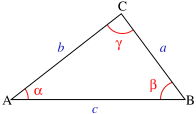
\includegraphics[scale=0.5]{Triangle_with_notations_2}

\[
 c^2 = a^2 + b^2 - 2ab\cos\gamma\,
\]
\[
 \frac{a}{\sin A} \,=\, \frac{b}{\sin B} \,=\, \frac{c}{\sin C} \,=\, D \!
\]


\subsection{Normal distribution}
\[
  f(x) = \frac{1}{\sigma\sqrt{2\pi}} e^{ -\frac{(x-\mu)^2}{2\sigma^2} }.
\]

\[
 \Phi(x)\; = \;\frac{1}{\sqrt{2\pi}} \int_{-\infty}^x e^{-t^2/2} \, dt
\]

\[
  F(x)\;=\;\Phi\left(\frac{x-\mu}{\sigma}\right)\
\]

\subsection{Factorial}

\begin{lstlisting}[language=C++]
1 1 2 6 24 120 720 5040 40320 362880 3628800 // 0..10
39916800 479001600 1932053504 // 11..13
\end{lstlisting}

\subsection{Primes}

\lstinputlisting[language=C++]{./lib/primes.cpp}

\subsection{Fibonacci}

\begin{lstlisting}[language=C++]
0 1 1 2 3 5 8 13 21 34 55 89 144 233 377 610 // 0..15
\end{lstlisting}

$F(0) = 0, F(1) = 1$

$F(n) = F(n - 1) + F(n - 2)$

\subsection{Combinatorics}

$C(n,0) = C(n,n) = 1$

$C(n,k) = C(n - 1, k - 1) + C(n - 1, k)$

\subsection{Catalan numbers}

\begin{lstlisting}[language=C++]
1 1 2 5 14 42 132 429 1430 4862 16796 // 0..10
\end{lstlisting}

\begin{enumerate*}
    \item $Cat(n)$ Count the number of distinct binary trees with $n$ vertices.
    \item Count number of expressions counting $n$ correctly matched pairs of parentheses.
    \item Count ways a convex polygon can be triangulated.
\end{enumerate*}

$Cat(0) = 1$

$Cat(n) = \frac{2(2n - 1)}{n + 1} * Cat(n - 1)$

\subsection{Powers of 2}
\begin{lstlisting}[language=C++]
1 2 4 8 16 32 64 128 256 512 1024 // 0..10
2048 4096 8192 16384 32768 65536  // 11..16
4294967296 4611686018427387904 // 32, 63
\end{lstlisting}

\subsection{Extended Euclid: Linear Diphantine Equation}
\lstinputlisting[language=C++]{./lib/extended_euclid.cpp}

\subsection{Cycle Finding}
\lstinputlisting[language=C++]{./lib/floydCycleFinding.cpp}

\subsection{Game Theory}

\subsubsection{Nim Game}

Two players take turns to remove objects from distinct heaps. On each turn, a player must remove at least one object and may remove any number of objects, but only from the same heap. For the starting player to win, $n_1 \text{\textasciicircum{}} ... \text{\textasciicircum{}} n_k \neq 0$. (bitwise xor)

\subsubsection{Josephus}
\lstinputlisting[language=C++]{./lib/josephus.cpp}


\subsection{Java BigInteger}

\lstinputlisting[language=Java]{./lib/bigInteger.java}

\lstinputlisting[language=Java]{./lib/catalan.java}

\subsection{2SAT}

Given 2-CNF $(x_1 \lor x_2) \land (\lnot x_3 \lor x_1) \lor ...$ is it satisfiable?

Rewrite $(a \lor b) \equiv (\lnot a \Rightarrow b) \equiv (\lnot b \Rightarrow a)$.

Build implication graph. Is satisfiable iff no variable is strongly connected with it's negation.  Try assignments for answer.

\section{DP}

\subsection{Longest Increasing Subsequence}
\lstinputlisting[language=C++]{./lib/lis.cpp}

\subsection{Knapsack}
\lstinputlisting[language=C++]{./lib/knapsack.cpp}


\section{Graph}

\subsection{Kruskal MST}
\lstinputlisting[language=C++]{./lib/kruskal.cpp}

\subsection{Bipartite check}
\lstinputlisting[language=C++]{./lib/is_bipartite.cpp}

\subsection{Maximum Bipartite Cardinality Matching}
\lstinputlisting[language=C++]{./lib/MCBM.cpp}

\subsection{Articulation points and bridges}
\lstinputlisting[language=C++]{./lib/articulationPointsAndBridge.cpp}

\subsection{Dijkstra}
\lstinputlisting[language=C++]{./lib/dijkstra.cpp}

\subsection{Dijkstra Timetable}
\lstinputlisting[language=C++]{./lib/dijkstra-timetable.cpp}

\subsection{Bellman Ford}
\lstinputlisting[language=C++]{./lib/bellman_ford.cpp}

\subsection{Euler Tour}
\lstinputlisting[language=C++]{./lib/euler.cpp}

\subsection{Edmond Karp}
\lstinputlisting[language=C++]{./lib/edmonds_karp.cpp}

\subsection{Maxflow Binblock}
\lstinputlisting[language=C++]{./lib/maxflow_binblock.cpp}

\subsection{Flood Fill}
\lstinputlisting[language=C++]{./lib/floodfill.cpp}

\subsection{Topological Sort}
\lstinputlisting[language=C++]{./lib/toposort.cpp}

\subsection{Strongly Connected Components}
\lstinputlisting[language=C++]{./lib/tarjanSCC.cpp}

\subsection{Chinese Postman}
\lstinputlisting[language=C++]{./lib/chinese_postman.cpp}


\section{String}

\subsection{Knuth-Morris-Pratt}
\lstinputlisting[language=C++]{./lib/kmp.cpp}

\subsection{Edit Distance}
\lstinputlisting[language=C++]{./lib/edit_distance.cpp}

\subsection{Longest Common Subsequence}
\lstinputlisting[language=C++]{./lib/lcs.cpp}

\subsection{Suffix Array}
\lstinputlisting[language=C++]{./lib/suffix_array.cpp}


\section{Geometry}

\subsection{Points and Lines}
\lstinputlisting[language=C++]{./lib/points_lines.cpp}

\subsection{Circles}
\lstinputlisting[language=C++]{./lib/circles.cpp}

\subsection{Triangles}
\lstinputlisting[language=C++]{./lib/triangles.cpp}

\subsection{Polygons}
\lstinputlisting[language=C++]{./lib/polygon.cpp}


\section{Misc}

\subsection{Interval Cover}
\lstinputlisting[language=C++]{./lib/interval-cover.cpp}

\subsection{Prefix Sum}
\lstinputlisting[language=C++]{./lib/prefix_sum.cpp}


\end{multicols}
\end{document}

